%%%% fs-run-time-experiments   Experiments

\label{fs-experiments-section}

We conducted a  series of experiments to estimate the performance of our  prototype. 
We used a problem of building an incremental inverted index as a stream processing benchmark  for the following reasons:
%% This task is chosen because it has the following properties:

\begin{itemize}
    \item It requires stateful operations that may cause overheads
    \item Computational flow contains network shuffle that can violate the ordering constraints %of some operations 
    enabling evaluation of our optimistic techniques.
    %Therefore, inverted index task can verify the performance of our optimistic approach
\end{itemize}

%It is worthwhile to mention that building inverted index can be considered as the halfway task between documents generation and searching. 
In the real-world, such scenario can be found in freshness-aware systems, e.g., news processing engines.

Building of inverted index % is implemented in terms of MapReduce transformations. 
%We 
starts with page mapping into the pairs {\it (word; word positions within the page)}, then  word positions are reduced by word into the single index update. 
%We assume the output of the stream to be change records of the inverted index structure, i.e., 
% each input page triggers the output of the corresponding updates. 
%
To avoid index inconsistencies, pairs {\it (word; word positions within the page)} must be ordered by page id and version before the update of inverted index state. 
%Otherwise, it is possible to obtain the inconsistent index, if there are multiple versions of the same document.  
 %
In \FlameStream\ this algorithm is implemented as a conversion of MapReduce transformation 
outlined in  section~\ref{fs-drifting}.
The index update record plays the role of an accumulator. 
%, and the final map produces the most recent changes of this structure if any.

The latency is defined as a (negated) time difference between entry of incoming data item and delivery of all output items generated in response to the incoming one.

%By the notion of {\it latency} we assume the time between two events: 

%\begin{enumerate}
%    \item Input page is taken into the stream
%    \item All the change records for the page leave the stream
%\end{enumerate}

Our experiments were performed on the cluster of Amazon EC2 micro instances with 1GB RAM and 1 core CPU. We used 10000 Wikipedia articles as a dataset. 

\subsection{Overhead and scalability}

%The proposed method can bring an additional overhead. Thus, it is essential to analyze the system's behavior under different configurations.
%
We take the ratio of  the total number of items at the barrier   to the number of the valid items among them as a key metric for the estimation of the overhead of our prototype and measure it for several system configurations.
%This value measures the extra cost of our approach.

The relation between the number of workers, the input  document  rate, and the  ratio is shown in Figure~\ref{overhead}. 
As expected, the peak of the ratio is achieved when the document per second rate is high, and the number of the nodes is low. This behavior can be explained by the fact that a few workers cannot effectively deal with such intensive load. Nevertheless, the proportion of invalid items reduces if the number of workers grows. 
%Under not very high pressure, 
The   overhead of  the optimistic technique under moderate pressure  is under 10\% for all  numbers of workers .
These results confirm that the ratio does not increase with the growth of the number of nodes.

\begin{figure}[ht]
  \centering
  \begin{minipage}[b]{.6\textwidth}
    \centering
    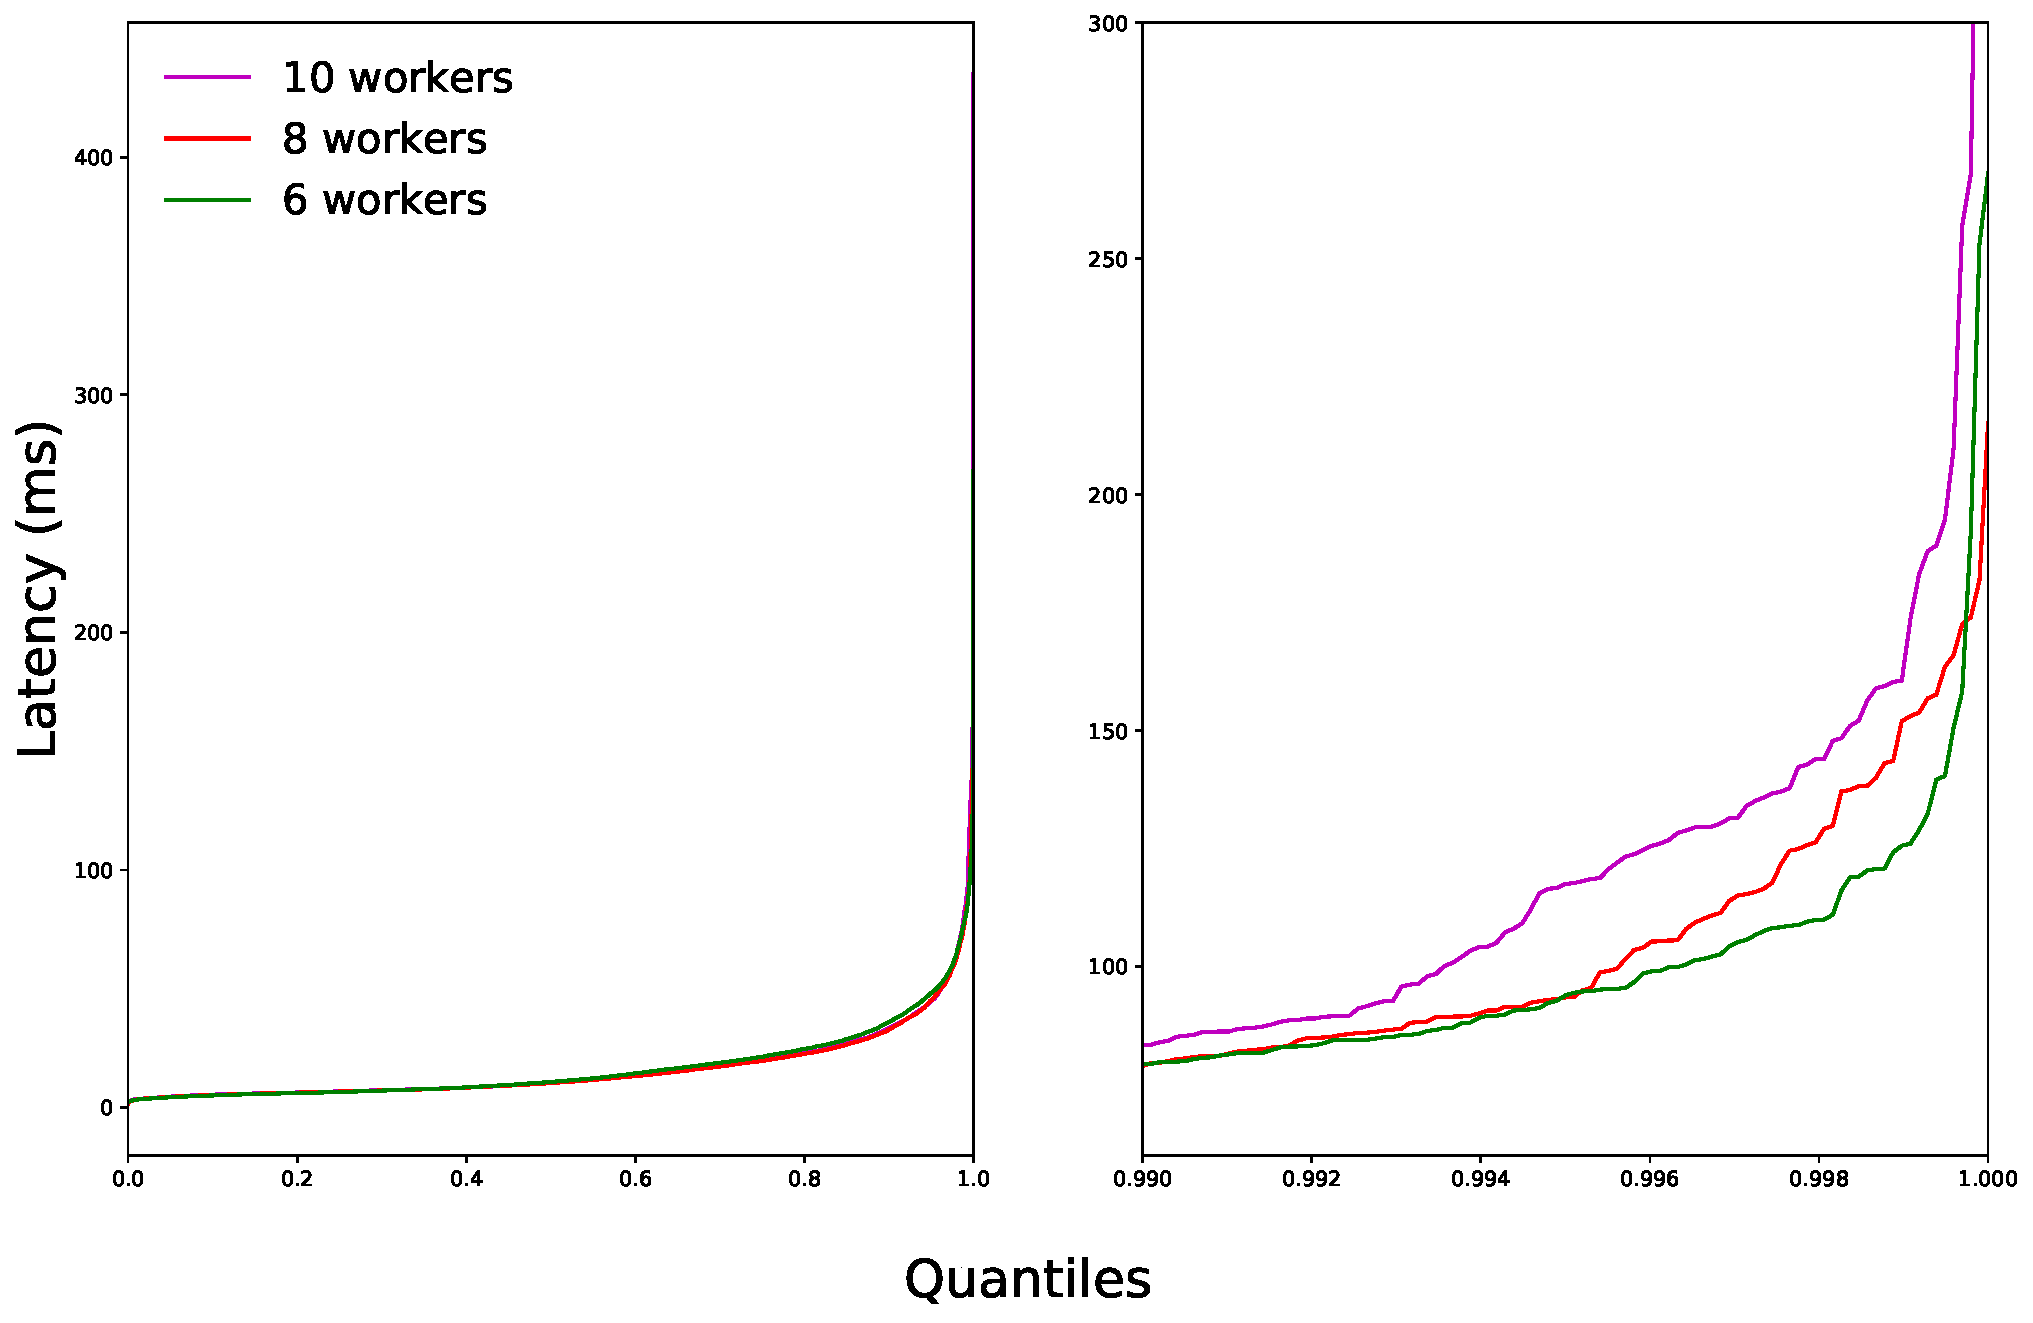
\includegraphics[width=\linewidth]{pics/fs-index-quantiles}
    \caption{FlameStream latency distribution. Left - the whole distribution, right - high quantiles}
    \label{fs-scalability}
  \end{minipage}%
  \begin{minipage}[b]{.40\textwidth}
    \centering
    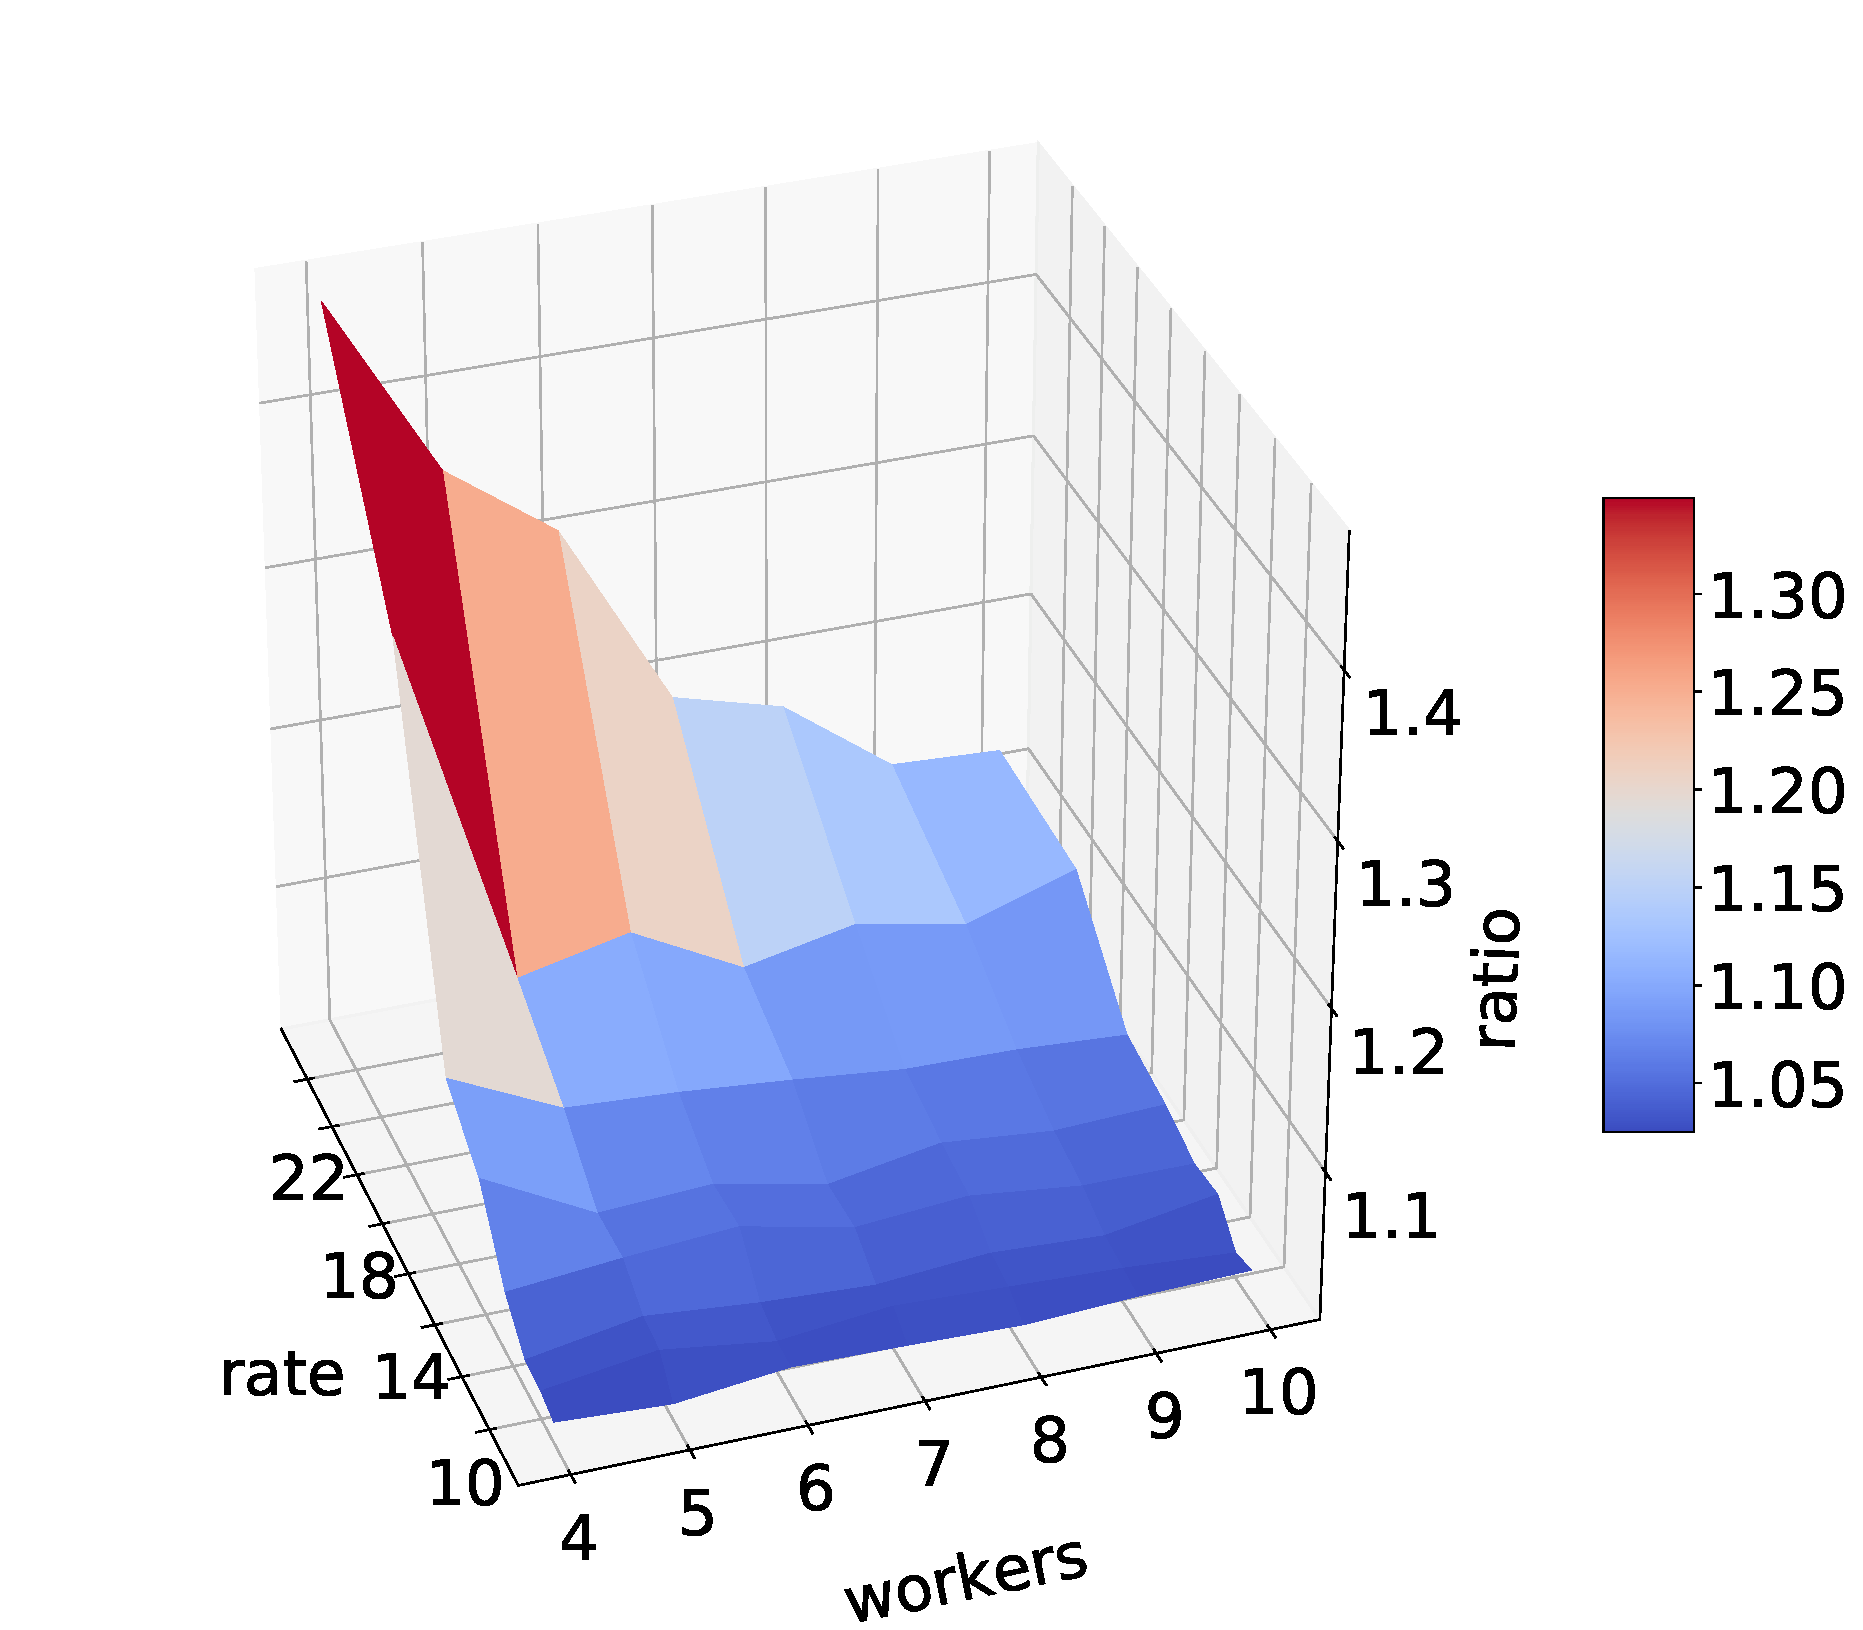
\includegraphics[width=\linewidth]{pics/overhead}
    \caption{The relation between the number of workers, the input document's average rate and the repair ratio}
    \label{overhead}
  \end{minipage}%
\end{figure}

The latencies of \FlameStream\ across multiple workers for the fixed document rate of 15 rps are shown in Figure~\ref{fs-scalability}. 
This experiment demonstrates that latency is stable  under  the growth in f the number of workers.
%
%Therefore, the most important conclusions of 
These experiments show that  the our method is scalable with proper  optimization of  the system setup.

\subsection{Performance Comparison with an Industrial Solution}

%One of the most important goals of the experiments is the performance comparison with an industrial solution regarding latency. 
Apache Flink is chosen for latency comparison in this experiment  because it is state-of-the-art stream processing system that provides similar functionality 
and achieves low latency in the real-world scenarios~\cite{S7530084}. 

For Apache Flink, the algorithm for building the inverted index is 
adopted 
by the usage of {\it FlatMapFunction} for map step and stateful {\it RichMapFunction} for reduce step and for producing the change records. 
Order enforcing before reduce is implemented using custom {\it ProcessFunction} that buffers all input until corresponding low watermark is received. Watermarks are sent after each document. The network buffer timeout is set to 0 to minimize latency.

% In this paper, 
We compare $50^{th}$, $75^{th}$, $95^{th}$, and $99^{th}$ percentile of distributions, which clearly represent the performance from the perspective of the users' experience.

The comparison of latencies between \FlameStream\ and Flink within 10 nodes and distinct document rates is shown in the (a) plot in Figure~\ref{fs-index-quantiles}. 
In this case, \FlameStream\ provides better  latency even under high load. 
These results confirm that optimistic approach for deterministic processing is able to yield  lower  latency than conservative techniques. 
The  reason for that  can be that Flink starts to update index only after the buffer before reduce stage is flushed, 
while  \FlameStream\ flushes its barrier right before data are delivered.
%is sent to a user, according to its optimistic nature. 
% At this moment, all corresponding computations have been already done. 
Low watermarks go along the stream and can be delayed by long-running operations, while acker processes ack messages independently. It is confirmed by (c) plot in Figure~\ref{fs-index-quantiles}, which compares  waiting time in Flink buffer and \FlameStream\ barrier.

\begin{figure}[ht]
  \centering
  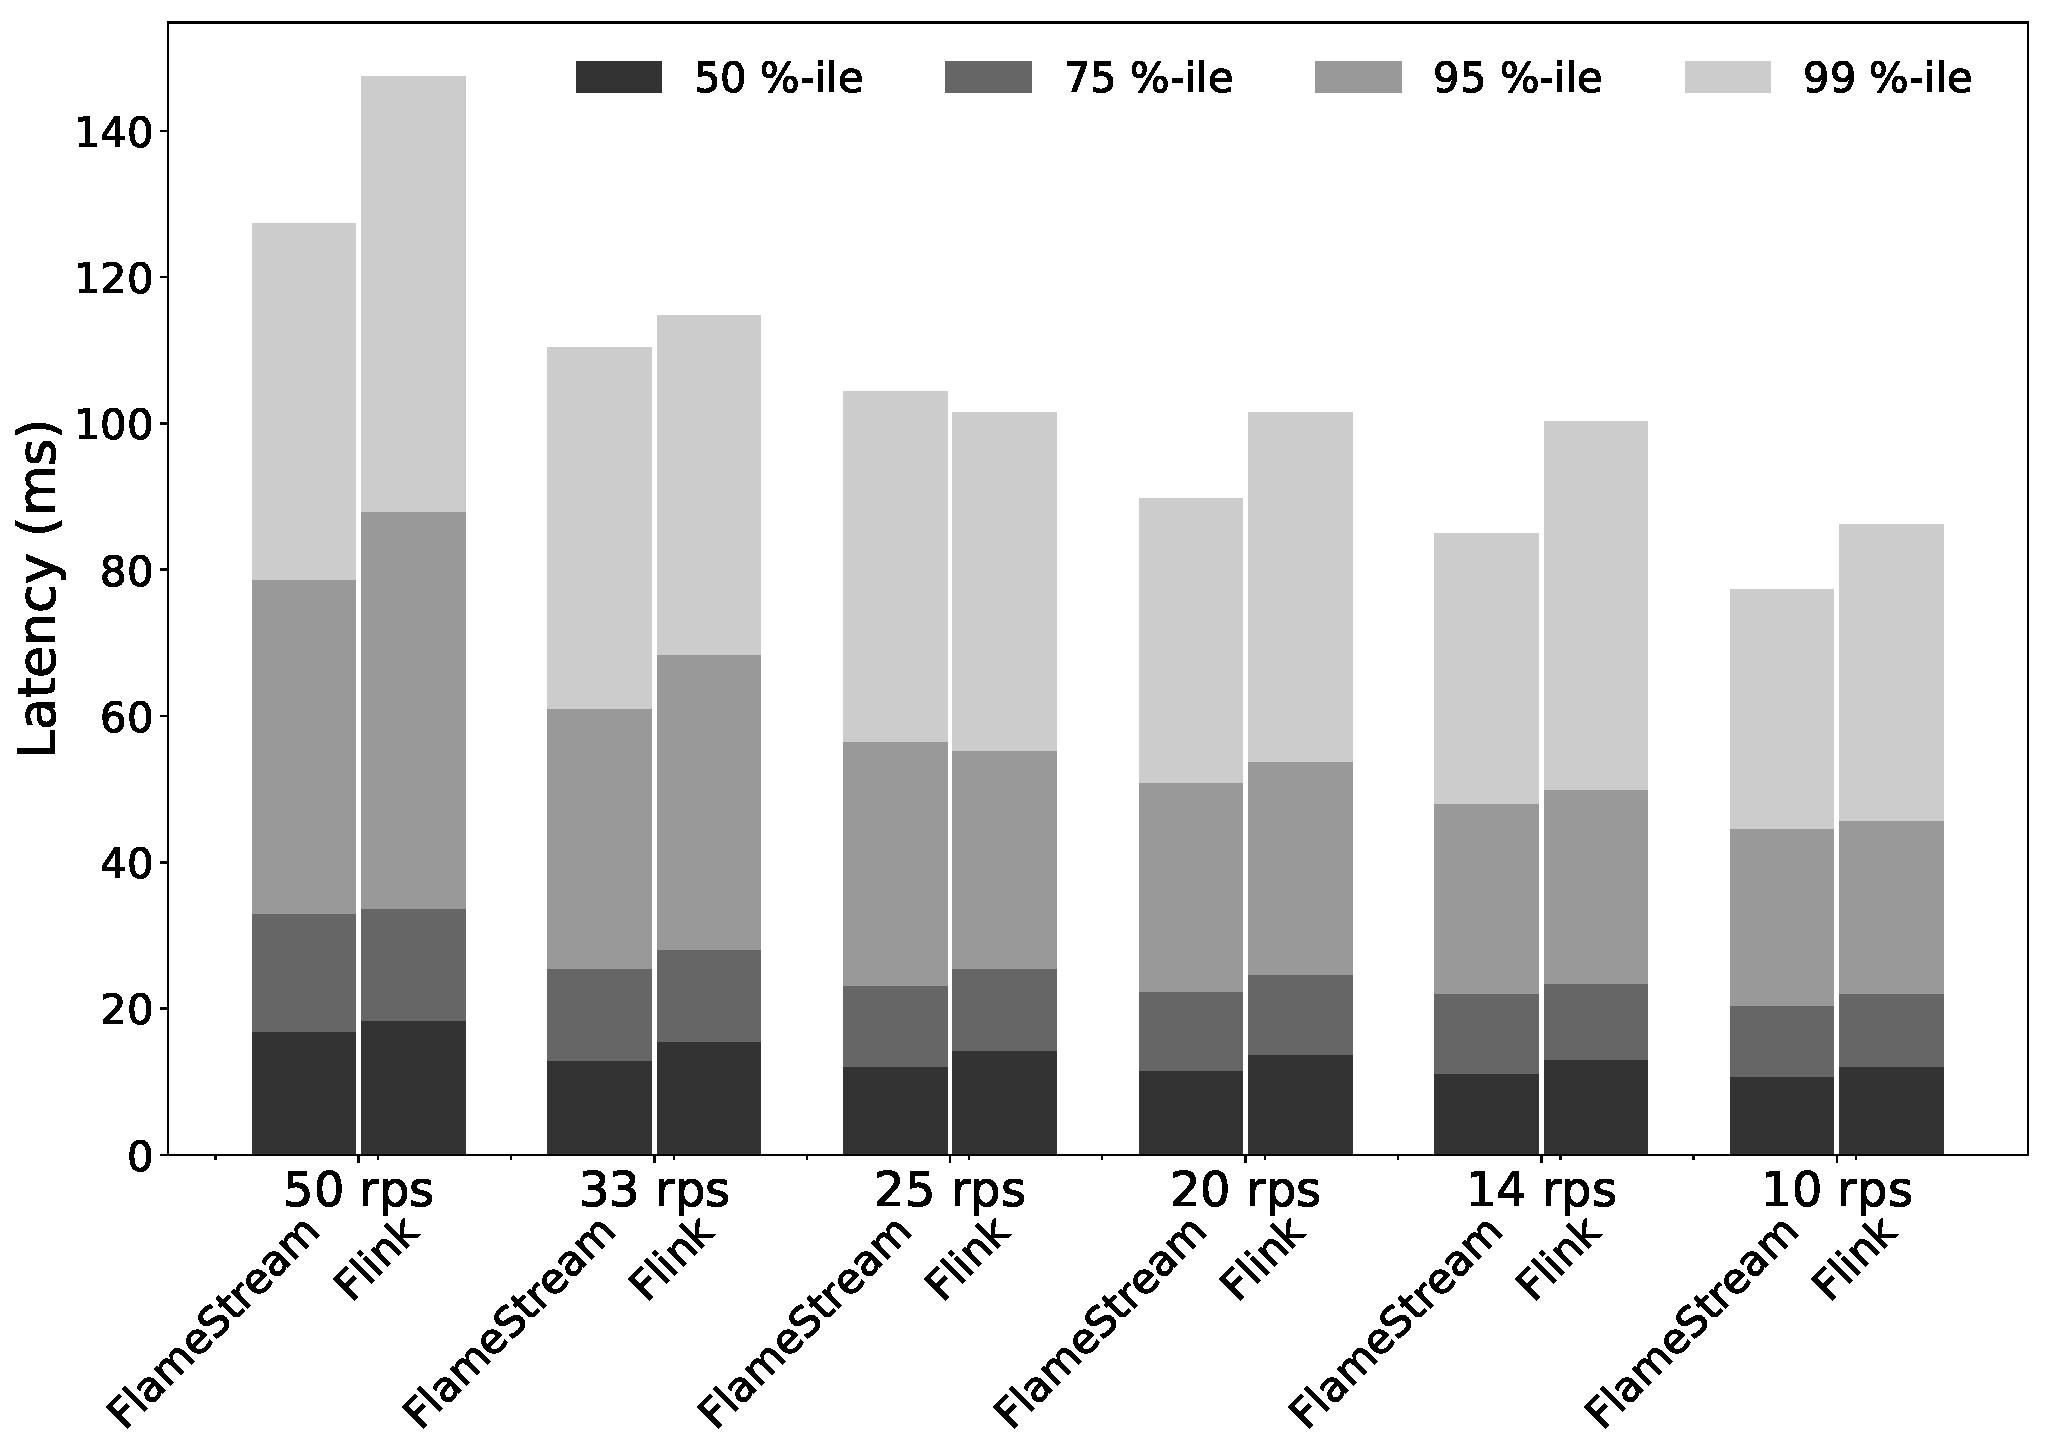
\includegraphics[width=\textwidth]{pics/comp-index-quantiles}
  \caption{The comparison in latencies between \FlameStream\ and Flink, (a) - 10 workers, (b) - 5 workers. (c) - the waiting time: Flink order enforcer vs. FlameStream barrier}
  \label {fs-index-quantiles}
\end{figure}

%However, there are conditions, which are not suitable for the optimistic approach. 

The (b) plot in Figure~\ref{fs-index-quantiles} 
compares  latencies between \FlameStream\ and Flink within 5 nodes and distinct document rates. 
Flink outperforms \FlameStream\ under extreme load. 
Such behavior follows from the fact that \FlameStream\ creates significant overhead under very high load.
% within a few computational units. 
This result evidently is in line with measurements of the overhead in Figure~\ref{overhead}. 
Nevertheless,  \FlameStream\ demonstrates better latency if the load is moderatee.

Thus, Flink can be more appropriate if there is a need to optimize computational resources under a fixed load, but the demands on latency are not very strict, or determinism is not required. \FlameStream\ is more relevant for cases when low latency and determinism are strict requirements, but an allocation of additional resources is not a problem.  


